\chapter{Clustering}

Clustering is a prime example of a problem typically associated with unsupervised learning.\footnote{In this work, both unsupervised as well as supervised approaches to clustering are explored.} \cite{xu_comprehensive_2015} even call clustering the most important question of unsupervised learning. The task is one of grouping objects into \name{clusters} such that the objects in any particular cluster are in some sense more similar to each other that to the objects from other clusters. Alternatively, the problem can be formulated as one finding a similarity measure on the object space such that the objects deemed to be similar actually are under the measure. Oftentimes, such a similarity measure is based on some distance function such as the Euclidean, Manhattan, Cosine, Minkowski or Mahalanobis (see \cite{mahalanobis_generalised_1936}) distance.

\section{Definition of clustering}
So far, the definition of terms such as "cluster" or "similar" has been left intuitive and vague. The reason for that is that there is no universal definition of what a cluster is. \cite{estivill-castro_why_2002} argues that there even should not be a universal definition as the clusters are, in a large part, on the eye of the beholder. Notwithstanding that, there is at least an informal definition provided by \cite{jain_algorithms_1988}:

\begin{enumerate}
	\item A cluster is a set of entities which are \textit{alike} and entities from different clusters are not alike.
	\item A cluster is an aggregation of points in the test space such that the \textit{distance} between any two points in the cluster is less than the distance between any point in the cluster and any point not in it.
	\item Cluster may be described as connected regions of a multi-dimensional space containing a relatively \textit{high density} of points, separated from other such regions by a region containing a relatively low density of points.
\end{enumerate}

Even with that definition, it is sometimes not clear what constitutes a cluster without some additional context. \cite{jain_algorithms_1988} presents figure \ref{fig:cluster-ambiguity} as an example.

\begin{figure}[h]
	\centering
	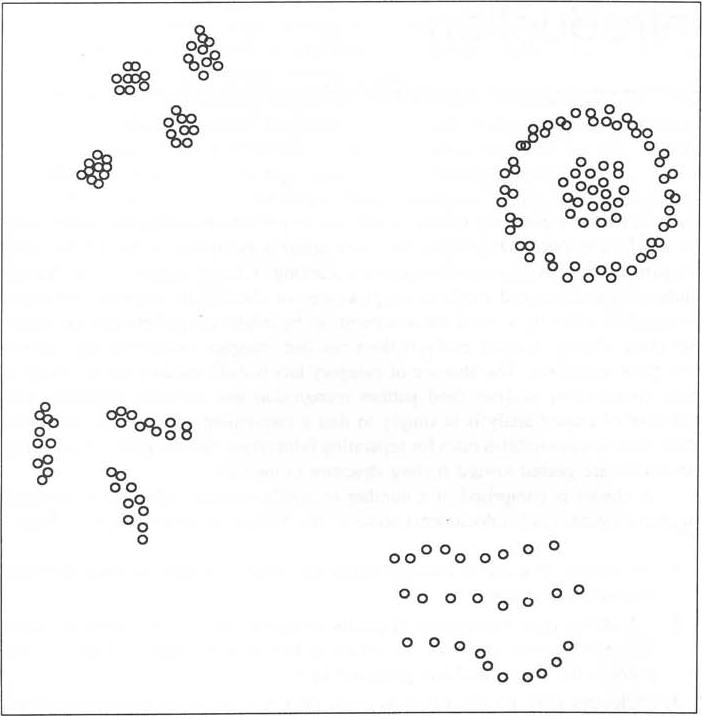
\includegraphics[width=0.9\textwidth]{images/cluster-ambiguity.png}
	\caption{An example of the ambiguity of clusters from \cite{jain_algorithms_1988}. At the global level, there are four clusters in the scatter plot. At a local level, or a lower similarity threshold, twelve clusters can be recognised however.}\label{fig:cluster-ambiguity}
\end{figure}

\cite{xu_comprehensive_2015} offers a comprehensive survey of different distance functions, similarity functions, evaluation indicators and clustering algorithms.
